% SC2203 --- Chapter 5: Pushdown Automata (0->100 ground-up)
\chapter{Pushdown Automata}
\label{ch:pushdown}

\begin{quote}
\emph{``A stack is counting you can pop.''} --- Add a stack to a finite control and $0^n1^n$ becomes recognisable; add only a stack and you exactly capture the context-free languages.
\end{quote}

\noindent\fbox{\parbox{\dimexpr\linewidth-2\fboxsep-2\fboxrule}{%
\textbf{From zero: we build here, no PDA assumed.} We define PDA from scratch---states, input, stack alphabet, push/pop---with pictures of stack height before formalism. CFG$\leftrightarrow$PDA equivalence is proved by two simulations. Only Ch.~4 required.}}
\vspace{0.4em}

\section*{Learning Outcomes}
After this chapter you will be able to:
\begin{enumerate}[label=(L\arabic*)]
    \item define PDA, instantaneous description and acceptance by final state / empty stack;
    \item simulate a PDA on $0^n1^n$ and on palindromes, explaining stack as counter;
    \item convert CFG to PDA (top-down) and PDA to CFG (triple construction) at high level;
    \item state the equivalence theorem PDA $\equiv$ CFG and outline both directions;
    \item explain why deterministic PDAs are strictly weaker and give an example.
\end{enumerate}

% ============================================================
\section{Pushdown Automata: Finite Control + Stack}
\label{sec:pda-def}
\emph{Intuition:} a DFA cannot remember $n$; a stack can. Push $0$s, pop one per $1$---if empty at the end, $n$ matched. The stack is LIFO: only the top is visible.

\begin{definition}[PDA]
A \emph{pushdown automaton} is $P=(Q,\Sigma,\Gamma,\delta,q_0,Z_0,F)$ where $Q$ finite states, $\Sigma$ input alphabet, $\Gamma$ stack alphabet, $q_0$ start, $Z_0\in\Gamma$ initial stack symbol, $F\subseteq Q$ accept, and $\delta:Q\times(\Sigma\cup\{\varepsilon\})\times\Gamma\to\mathcal{P}(Q\times\Gamma^*)$ finite. $(p,\gamma)\in\delta(q,a,X)$ means: in $q$ reading $a$ (or $\varepsilon$) with top $X$, go to $p$ and replace $X$ by $\gamma$ (push, pop, or replace).
\end{definition}

An \emph{ID} is $(q,w,\gamma)$: state, remaining input, stack contents (left = top). Step $(q,aw,X\beta)\vdash(p,w,\gamma\beta)$ if $(p,\gamma)\in\delta(q,a,X)$; also $\varepsilon$-moves $(q,w,X\beta)\vdash(p,w,\gamma\beta)$. Acceptance: by \emph{final state} ($q\in F$ after consuming all input, stack anything) or by \emph{empty stack} (stack becomes $\varepsilon$). The two modes are equivalent (add new bottom marker and draining states).

% TikZ 1: PDA schematic with stack
\begin{figure}[h]
\centering
\begin{tikzpicture}[scale=0.82,every node/.style={font=\scriptsize}]
\draw[thick,fill=blue!10,rounded corners=4pt] (0,0) rectangle (2.4,2.2);
\node[font=\footnotesize\bfseries] at (1.2,1.9) {Finite control};
\node[draw,circle,fill=white,minimum size=0.6cm] at (1.2,1.2) {$q$};
\node[font=\tiny] at (1.2,0.5) {state $q$};
\draw[thick,fill=green!14,rounded corners=3pt] (0,-1.1) rectangle (2.4,-0.55);
\node[font=\tiny] at (1.2,-0.82) {Input: $a_1a_2\cdots\rhd$};
\draw[->,thick,blue!60!black] (1.2,0.02)--(1.2,-0.48) node[midway,right,font=\tiny] {read $a$};
% stack
\draw[thick,fill=orange!18,rounded corners=3pt] (4.2,-0.6) rectangle (6.0,2.2);
\node[font=\footnotesize\bfseries] at (5.1,1.9) {Stack $\Gamma^*$};
\foreach \i/\sym in {1/Z_0,2/0,3/0} {\pgfmathsetmacro{\y}{-0.15+0.55*\i}\draw[thick,fill=white] (4.35,\y) rectangle (5.85,\y+0.45); \node[font=\tiny] at (5.1,\y+0.22) {$\sym$};}
\node[font=\tiny] at (5.1,1.15) {top $\to$};
\draw[->,thick,red!70!black] (2.5,1.0)--(4.15,1.3) node[midway,above,font=\tiny] {pop $X$ / push $\gamma$};
\draw[->,thick,red!70!black] (4.15,0.9)--(2.5,0.7);
\node[font=\tiny,fill=yellow!12,rounded corners=2pt] at (3.2,-1.35) {LIFO: only top accessible};
\end{tikzpicture}
\caption{PDA: finite control points to input head and stack top; a transition $\delta(q,a,X)\ni(p,\gamma)$ replaces top $X$ by $\gamma$ while moving the input head if $a\neq\varepsilon$.}
\label{fig:pda-schematic}
\end{figure}

\begin{example}[PDA for $L=\{0^n1^n\mid n\ge0\}$ by empty stack]
$\Gamma=\{Z_0,0\}$; push $0$ for each $0$ input, pop one $0$ per $1$. Sketch: $\delta(q_0,0,Z_0)=\{(q_0,0Z_0)\}$, $\delta(q_0,0,0)=\{(q_0,00)\}$, $\delta(q_0,1,0)=\{(q_1,\varepsilon)\}$, $\delta(q_1,1,0)=\{(q_1,\varepsilon)\}$, $\delta(q_1,\varepsilon,Z_0)=\{(q_f,\varepsilon)\}$. Trace $0011$: stack $Z_0\to0Z_0\to00Z_0\xrightarrow{1}0Z_0\xrightarrow{1}Z_0\xrightarrow{\varepsilon}\varepsilon$ accept. Non-member $001$ blocks with stack $0Z_0\neq\varepsilon$.
\end{example}

% TikZ 2: stack height vs input for 0^n1^n
\begin{figure}[h]
\centering
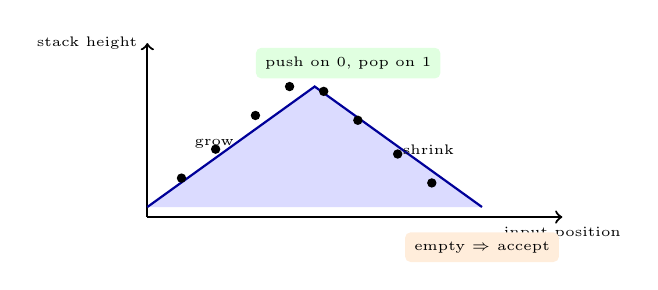
\begin{tikzpicture}[scale=0.85,every node/.style={font=\scriptsize}]
\draw[->,thick] (0,0)--(6.2,0) node[below,font=\tiny] {input position};
\draw[->,thick] (0,0)--(0,2.6) node[left,font=\tiny] {stack height};
\fill[blue!14] (0,0.15) -- (2.5,1.95) -- (5.0,0.15) -- cycle;
\draw[thick,blue!60!black] (0,0.15)--(2.5,1.95)--(5.0,0.15);
\foreach \x/\lbl in {0.6/0,1.2/0,1.9/1,2.5/1,3.1/1,3.7/1,4.4/1,5.0/\varepsilon} {\fill ( \x*0.85, {0.15+ ( \x<3 ? \x*0.72 : (5.5-\x)*0.72 ) } ) circle (2pt);}
\node[font=\tiny,fill=green!12,rounded corners=2pt] at (3.0,2.3) {push on $0$, pop on $1$};
\node[font=\tiny] at (1.0,1.1) {grow};
\node[font=\tiny] at (4.2,1.0) {shrink};
\node[font=\tiny,fill=orange!14,rounded corners=2pt] at (5.0,-0.45) {empty $\Rightarrow$ accept};
\end{tikzpicture}
\caption{Stack height mirrors the count: rises $n$ steps on $0$s, falls $n$ steps on $1$s; mismatch leaves stack non-empty or blocks on empty pop.}
\label{fig:stack-height}
\end{figure}

\begin{example}[Palindromes need nondeterminism]
$L=\{ww^R\mid w\in\{0,1\}^*\}$ (even palindromes) PDA: push input until nondeterministically guess the middle, then pop and match. Formally $q_0$ pushes $0,1$; $\varepsilon$-move $q_0\to q_1$ (switch to popping); in $q_1$, $\delta(q_1,0,0)=\{(q_1,\varepsilon)\}$ etc.; $w\in L$ iff some guess of middle position matches. No DPDA recognises all palindromes (deterministic cannot guess centre).
\end{example}

\begin{remark}[Acceptance modes unified]
To convert empty-stack $\to$ final-state, add fresh $q_f$ accepting and $\varepsilon$-moves draining stack to $q_f$; to convert final-state $\to$ empty-stack, add bottom marker $X_0$ and a draining phase that pops everything after entering $F$. Hence we may assume whichever is convenient in proofs.
Both conversions add at most one new state and one stack symbol, so size blow-up is constant.
\end{remark}

\begin{example}[Code: PDA simulator (nondeterministic BFS)]
\begin{lstlisting}[language=Python]
def accepts_pda(pda, w):
    from collections import deque
    frontier = deque([(pda.q0, 0, (pda.Z0,))])  # (state, pos, stack tuple top-first)
    visited=set()
    while frontier:
        q,pos,stk = frontier.popleft()
        if pos==len(w) and q in pda.F:  # accept by final state
            return True
        if (q,pos,stk) in visited: continue
        visited.add((q,pos,stk))
        top = stk[0] if stk else None
        for (a,X), moves in pda.delta.items():
            if X != top: continue
            if a != '' and (pos>=len(w) or w[pos]!=a): continue
            for p,gamma in moves:
                npos = pos+1 if a!='' else pos
                nstk = tuple(gamma)+stk[1:] if gamma else stk[1:]
                frontier.append((p,npos,nstk))
    return False
\end{lstlisting}
BFS over IDs explores nondeterministic branching; $\varepsilon$-moves keep \texttt{pos} unchanged, so bound depth or detect loops via visited.
\end{example}

% ============================================================
\section{Equivalence: CFG $\Leftrightarrow$ PDA}
\label{sec:cfg-pda-equiv}
\begin{theorem}[CFG $\equiv$ PDA]
$L$ is context-free iff some PDA recognises $L$ (by final state or empty stack). Conversions are effective.
\end{theorem}

\emph{Intuition for CFG $\to$ PDA (top-down):} PDA simulates leftmost derivation on its stack: stack holds the ``yet-to-derive'' suffix. If top is variable $A$, nondeterministically replace it by $\alpha$ for some $A\to\alpha$ ($\varepsilon$-move). If top is terminal $a$, match it against next input symbol and pop on equality. Start with $SZ_0$? Actually start symbol $S$ on stack above $Z_0$; accept when stack empties after matching input. This is how LL parsers work.

% TikZ 3: CFG->PDA top-down simulation
\begin{figure}[h]
\centering
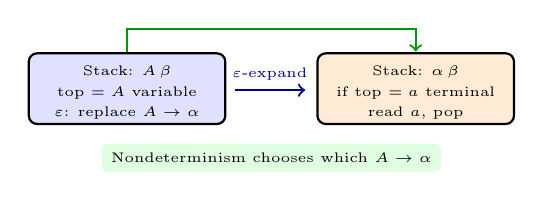
\begin{tikzpicture}[scale=0.78,every node/.style={font=\scriptsize}]
\draw[thick,fill=blue!12,rounded corners=3pt] (0,0) rectangle (3.2,1.15);
\node[font=\tiny] at (1.6,0.85) {Stack: $A\,\beta$};
\node[font=\tiny] at (1.6,0.50) {top $=A$ variable};
\node[font=\tiny] at (1.6,0.18) {$\varepsilon$: replace $A\to\alpha$};
\draw[->,thick,blue!60!black] (3.35,0.55)--(4.5,0.55) node[midway,above,font=\tiny] {$\varepsilon$-expand};
\draw[thick,fill=orange!16,rounded corners=3pt] (4.7,0) rectangle (7.9,1.15);
\node[font=\tiny] at (6.3,0.85) {Stack: $\alpha\,\beta$};
\node[font=\tiny] at (6.3,0.50) {if top $=a$ terminal};
\node[font=\tiny] at (6.3,0.18) {read $a$, pop};
\node[font=\tiny,fill=green!12,rounded corners=2pt] at (3.95,-0.55) {Nondeterminism chooses which $A\to\alpha$};
\draw[->,thick,green!60!black] (1.6,1.18)--(1.6,1.55)--(6.3,1.55)--(6.3,1.18);
\end{tikzpicture}
\caption{CFG$\to$PDA: expand variables via $\varepsilon$-moves; match terminals against input. Every leftmost derivation corresponds to a PDA computation and vice versa.}
\label{fig:cfg-to-pda}
\end{figure}

\emph{Intuition for PDA $\to$ CFG (triple construction):} variable $[pXq]$ means ``from state $p$ with stack top $X$, PDA can reach $q$ and pop $X$ (net effect: stack height unchanged beyond $X$)''. Productions: if $\delta(p,a,X)\ni(r,\varepsilon)$ then $[pXr]\to a$; if $\delta(p,a,X)\ni(r,YZ)$ then $[pXq]\to a[rY s][sZq]$ for all $s,q$. Start $S\to[q_0Z_0q]$ for all $q\in F$. Induction shows $[pXq]\Rightarrow^*w$ iff $(p,w,X)\vdash^*(q,\varepsilon,\varepsilon)$. Details are standard but lengthy; the idea is the stack discipline forces nested intervals.

\begin{example}[PDA$\to$CFG on $\{0^n1^n\}$]
Triple variables include $[q_0Z_0q_f]$, $[q_00q_1]$, etc. From $\delta(q_0,0,0)=(q_0,00)$ we get $[q_00s]\to0[q_00t][t0s]$; from $\delta(q_1,1,0)=(q_1,\varepsilon)$ we get $[q_10q_1]\to1$. The resulting grammar generates $0^n1^n$ after eliminating useless variables, essentially recovering $S\to0S1\mid\varepsilon$.
\end{example}

\begin{remark}[Determinism]
DPDA: $\delta(q,a,X)$ has at most one move and at most one of $\delta(q,a,X)$, $\delta(q,\varepsilon,X)$ defined (no choice). DPDA $\subsetneq$ PDA $=$ CFG: $L=\{a^nb^n\}\cup\{a^nb^{2n}\}$ is CFL but no DPDA recognises it (needs to decide which block count after reading $a$'s). DPDA languages (DCFLs) are closed under complement but not union. LR grammars correspond to DPDAs.
\end{remark}

\begin{example}[DPDA vs.\ PDA: $\{wcw^R\}$ is deterministic]
With centre marker $c$, PDA is deterministic: push $w$ until $c$, then pop and match. Formal DPDA: in $q_0$, push $0,1$ on $0,1$; on $c$ go to $q_1$; in $q_1$, $\delta(q_1,0,0)=(q_1,\varepsilon)$, $\delta(q_1,1,1)=(q_1,\varepsilon)$. Acceptance by final state at bottom $Z_0$. Removing $c$ (palindromes $ww^R$) forces nondeterminism---no DPDA exists, proving DCFL $\neq$ CFL.
\end{example}

\begin{example}[Stack as counter with two symbols]
$L=\{a^ib^jc^k\mid i=j\text{ or }j=k\}$ has PDA that nondeterministically guesses which equality to check: branch $1$ pushes $a$'s then pops on $b$'s and ignores $c$'s; branch $2$ ignores $a$'s then pushes $b$'s and pops on $c$'s. Either branch suffices, so union is CFL despite no single counter handling both equalities.
\end{example}

% ============================================================
\section{Closure and Decidability for CFLs via PDAs}
\label{sec:pda-closure}
CFLs are not closed under $\cap$/complement, but $L\cap R$ with $R$ regular \emph{is} CFL (product of PDA and DFA: keep DFA state in PDA control). This preserves decidability of emptiness ($L(G)=\emptyset$? check if $S$ derives a terminal string) and membership (CYK $O(n^3)$), but universality, equivalence, and inclusion become undecidable (via halting, Ch.~7). The triple construction also shows every CFL is accepted by empty stack with a single-state PDA? Actually $2$ states suffice.

\begin{theorem}[Regular intersection]
If $L$ CFL and $R$ regular then $L\cap R$ CFL. Construction: $P'=(Q\times Q_R,\Sigma,\Gamma,\delta', (q_0,r_0), Z_0, F\times F_R)$ where $\delta'((q,r),a,X)\ni((p,\delta_R(r,a)),\gamma)$ for each $(p,\gamma)\in\delta(q,a,X)$. Then $L(P')=L(P)\cap R$.
\end{theorem}
The construction mirrors the DFA product in Ch.~2; the DFA component is encoded in the finite control, leaving the stack untouched. Hence regular constraints do not add stack power.

\begin{example}[Using $L\cap R$ to prove non-CFL]
$L=\{a^nb^nc^n\mid n\ge0\}$ is not CFL, but $L_1=\{a^ib^jc^k\mid i=j\text{ or }j=k\}$ is. Intersect $L_1$ with regular $a^*b^*c^*$ does nothing; but $L_1\cap a^*b^*c^*$ already shows why closure matters. For $L=\{ww\mid w\in\{0,1\}^*\}$, intersect with $0^*1^*0^*1^*$ to force shape, then pump.
\end{example}

\begin{remark}[Why PDAs are nondeterministic by default]
Unlike DFAs, deterministic PDAs are strictly weaker. The subset-like construction fails because stacks cannot be subset-combined: two stack contents $00$ and $11$ cannot be merged into a single ``super-stack''. Hence we keep PDAs nondeterministic when proving CFG$\equiv$PDA.
\end{remark}

% ============================================================
\section{Chapter Notes}
Oettinger (1961) and Sch\"utzenberger proved CFG$\equiv$PDA; Ginsburg--Greibach systematised the triple construction. Evey (1963) optimised state count.
For parsing, LL corresponds to top-down PDA simulation, LR to bottom-up (handle) simulation; Knuth's LR theorem characterises DCFLs as exactly the deterministic languages.
The single-stack restriction is essential: two stacks give Turing power (Ch.~6); one stack plus nondeterminism gives exactly CFLs.
Hopcroft--Ullman gives the full triple proof; Sipser presents a streamlined version. Implement the CFG$\to$PDA conversion and test on $0^n1^n$ to see stack growth.

% ============================================================
\section{Exercises}
\label{sec:ch05-exercises}
Nondeterminism, stack invariants, and the two simulations are the testable skills; E5.5 separates DCFL from CFL.
Try implementing the $wcw^R$ DPDA deterministically before attempting palindromes nondeterministically.
For E5.4, eliminate useless variables: a variable is useful only if reachable from $S$ and can derive a terminal string.
\begin{enumerate}[label=E5.\arabic*, leftmargin=*, itemsep=0.8em]
\item \textbf{PDA trace.} Simulate the $0^n1^n$ PDA on $0011$ and $0101$; list IDs $(q,w,\gamma)$ step by step and indicate where nondeterminism would branch for palindromes.
\item \textbf{Design PDAs.} Give PDA (by final state) for $L=\{0^i1^j\mid i\le j\}$ and for $L=\{a^nb^nc^m\mid n+m\text{ even}\}$; explain stack invariant ``height $=$ excess $0$s''.
\item \textbf{CFG $\to$ PDA.} Convert $S\to0S1\mid\varepsilon$ to a top-down PDA: list $\Gamma$, $Z_0$, and each $\delta$ entry; trace $01$ and show the stack content after each expand/match.
\item \textbf{PDA $\to$ CFG.} Apply triple construction to the $1$-state PDA for $\{a^n b^n\}$ with single control $q$ and $\Gamma=\{Z_0,X\}$; simplify to $S\to aSb\mid\varepsilon$ after removing useless variables.
\item \textbf{Determinism gap.} Prove no DPDA accepts $L=\{a^nb^n\}\cup\{a^nb^{2n}\}$: assume DPDA exists, show it must commit after $a^n$ without knowing whether $b^n$ or $b^{2n}$ follows, then fool it with a distinguishing continuation.
\end{enumerate}
% Hint: for DPDA proofs, use the fact that the stack content after reading $a^n$ is determined, and the suffix $b^n$ vs.\ $b^{2n}$ forces a premature decision.
% End of Chapter 5
